\documentclass[tikz, border=3.14mm]{standalone}
\usepackage{circuitikz}

\begin{document}
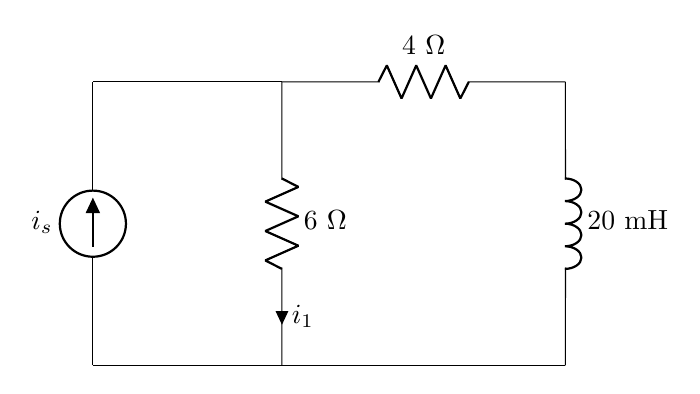
\begin{tikzpicture}[american, scale=1.2]
    % Main current source at the left
    \draw (0,0) to[I, l=$i_s$] (0,3); % Arrow points up (0 -> 3)
    
    % Horizontal wire to first branch
    \draw (0,3) -- (2,3);
    \draw (0,0) -- (2,0);
    
    % First vertical branch: 6 ohm resistor
    \draw (2,3) to[R, l=6~$\Omega$, i=$i_1$] (2,0);
    
    % Top horizontal branch (North Branch) with 4 ohm resistor
    \draw (2,3) to[R, l=4~$\Omega$] (5,3);
    
    % Second vertical branch: 20 mH inductor
    \draw (5,3) to[L, l=20~mH] (5,0);
    
    % Completion of the bottom wire
    \draw (5,0) -- (2,0);
    
\end{tikzpicture}
\end{document}
